\chapter{Introduction}

\section{Cyber-physical system}
Cyber-physical systems are a special type of real-time systems that combine a microcontroller or software program, represented by a discrete state machine, with one or more sensors that interact with a physical variable. Examples of this type of environment are the on-board computers that regulate the speed of a vehicle, or the autopilot that controls the altitude and trajectory of an aircraft.

Ensuring the proper functioning of these platforms is crucial, since a malfunction leads to a reduction in user comfort or even the loss of human lives. One way to ensure this is through the use of formal verification techniques. Runtime verification techniques \cite{STTT_RV_21} implement a monitor that monitors that the current execution meets specified requirements. Monitors act as keepers, alerting the user when execution deviates from desired behavior and even implementing countermeasures to reverse that fact and redirect the system back to a healthy state.

There are various formalisms to define desired and undesired behaviors. Functional requirements can be expressed operationally, through some kind of finite state automaton, or declaratively, through a logical-mathematical description. Within this second category, temporal logic is a type of modal logic that expresses properties about a particular \emph{state} of the system, or about the \emph{paths} (ie, sequence of states) that it traverses. In this work we will use Signal Temporal Logic \cite{STL}, a type of temporal logic focused on the analysis of analog signals.

\section{Objectives}

The objectives of this project are:

\begin{itemize}
\item Extend the capabilities of temporal logic to express properties involving \textit{trends} (derivatives), or \textit{accumulations} (integrales), 
\item Implement these new logical operators in current software tools, and
\item Provide a friendly user interface that facilitates interaction with said tools.
\end{itemize}


In particular, the project objectives have been translated into concrete contributions to the following pre-existing software tools:

\begin{itemize}
\item textbf{STLEval} \cite{StlEval}: It is a tool capable of processing STL specifications and evaluating them on a real signal. It has received the implementation of the new time-logic operators that calculate derivatives and integrals on a signal.
\item textbf{STLEval} \cite{StlEval}: It is a mining library that learns the (in)valid configurations of the monitored system expressed as templates or parametric specifications in STL.
ParetoLib internally interfaces with STLEval for the execution of the calculations. It has received an update of the STLEval binaries and DLL libraries which package together with the rest of the library, as well as the graphical user interface. The new GUI allows to interact both with the learning library and indirectly with the STLEval tool.
\end{itemize}

\section{Document Organization}

The document is divided into X chapters. In the chapter \ref{cha:stl} we will detail the semantics and implementation of the new logical operators. The \ref{cha:gui} chapter is dedicated to the new graphical user interface. We continue with the most relevant conclusions of the project in the chapter \ref{cha:concl}. Finally $\ldots$.

\section{Time schedule and effort}
This project lasted 8 months and was carried out by two part-time students, Dmytro Vernyuk (GII) and Javier Romero Flores (GIC), with an average dedication of 3 hours per day. The students have been tutored by José Ignacio Requeno through weekly meetings. Approximately 1300 lines of code have been modified or created, which are distributed between the two updated software tools and the new graphical user interface.
graphical user interface. The code developed in this project can be consulted in the new functionalities of the corresponding web repositories (\textit{derivative} branch of STLEval and \textit{GUI} branch of ParetoLib).

The project started on September 13, 2021, and has consisted of 4 phases:


\subsection{First - Research}
The project started with a first phase of research, where we dedicated ourselves to theoretical knowledge necessary for the work: reading information about what is temporal logic and the main difference with other modal logics.
We resorted both to the material provided by the instructor and to the external material available to learn the main definitions and basic syntax.
This was the most complicated part of the whole work not only because of the theoretical difficulty of the specialized information in the field of 
but also because of the paradigm shift involved in understanding the main concept of this logic: that an assertion can become a negation depending on the instant at which the expression is evaluated.


\subsection{Second - Documentation}
After acquiring the previous theoretical knowledge necessary for the understanding of the functionalities to be implemented, we continued with the reading of the documentation of the libraries and software tools to be extended: their software architecture and class hierarchy. We devoted a great deal of effort to study the definition of the derivation and integration operators proposed in the scientific literature, and their subsequent coding and incorporation into the STLEval software tool.

\subsection{Third - Implementation}
We implemented the operations of derivation and integration of time signals in the STLEval software tool. We completed this task with a set of tests on time signals with \textit{benign} characteristics that facilitated us to run validation tests: for example, the integral of a periodic signal (sinusoidal or triangular) symmetric about the horizontal axis should be zero in  certain intervals.

\subsection{Fourth - Design and Completion}
As a last task we implemented the graphical interface of the application, starting from a first sketch that we stabilized after two meetings. The most complicated task of this process was the connection between the different components of the interface with the methods of the STLEval and ParetoLib tools, which execute all the program logic.

The connection with STLEval was made through a pre-existing API in C++ that was already integrated in Python through the ParetoLib library. This fact, the possibility of accessing both the ParetoLib mining library and the STLEval tool indirectly, motivated the choice of Python as the programming language for the design of the user windows. The ease of use of the language as well as the number of auxiliary libraries for data processing with which to extend the functionalities of the interface in the future also contributed to this decision.

\section{Team Organization}
Due to the theoretical difficulty of this project, we decided to carry out the tasks jointly: all the sections of this project, except for the documentation work, were carried out at the same time by both members of the team.
The planning coincides with the phases of the project, the exact dates are shown in the following chart:

\begin{figure}
\centering
  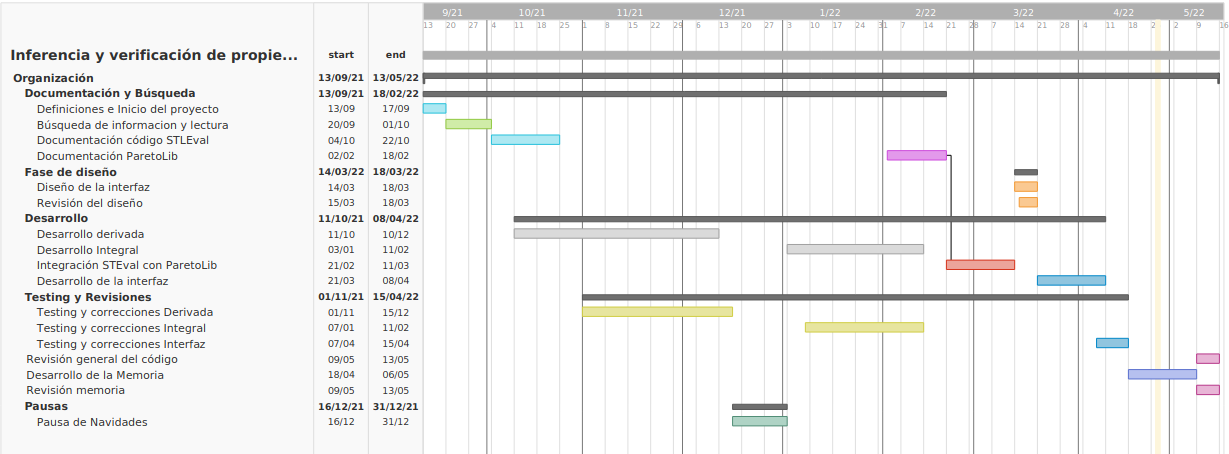
\includegraphics[width=.9\linewidth ,angle = 90,scale = 1.2]{images/gant}
\caption{Diagrama de Gantt.}
\label{fig:gant}
\end{figure}